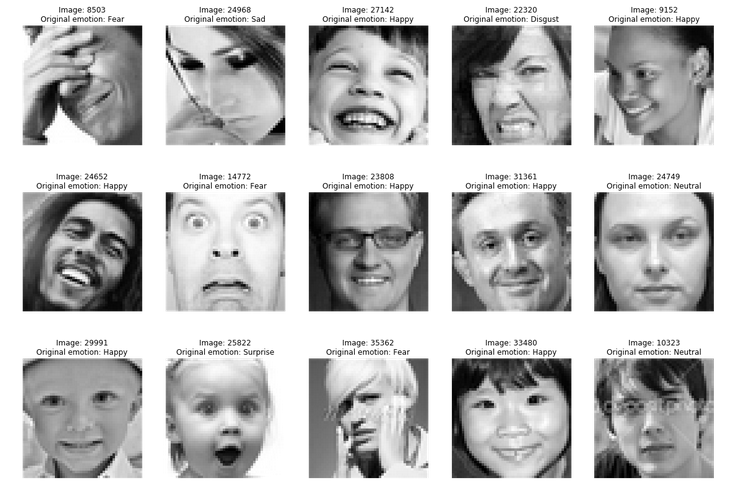
\includegraphics[scale=0.75]{images/ferCover.png}
\\Data that we got is in one *.csv file with almost 36 thousands rows and two columns:
\begin{itemize}
  \item number of emotion \\
        in range 0 - 6
        \begin{itemize}
          \item 0 - angry
          \item 1 - disgust
          \item 2 - fear
          \item 3 - happy
          \item 4 - sad
          \item 5 - surprise
          \item 6 - neutra
        \end{itemize}
  \item string of pixels \\
        pixels are in one long string (2304 of them), they are in grayscale 0 - 255.\\
\end{itemize}
This pixels will be processed depending on the model.\\
Training part has 28708 images, testing only 7178.